\section{Representasi Data Finansial}
Pasar finansial merupakan sistem yang dinamis namun pergerakannya tidak bersifat acak murni karena dipengaruhi oleh interaksi strategis antar pelaku pasar yang terstruktur \cite{schwert_chapter_2003}. Untuk mengidentifikasi peluang profitabilitas dari dinamika tersebut, investor menerapkan Metodologi analisis kualitatif dan teknikal untuk mengolah informasi yang relevan dari fluktuasi harga historis dan memanfaatkannya untuk memprediksi pergerakan harga di masa depan \cite{freitas_game_2024}. Representasi data finansial dalam memetakan perilaku kolektif para agen ekonomi \textit{price noise} menjadi bentuk visual bagi para analis pasar profesional. Data mentah tersebut diproses menjadi data yang terstruktur sehingga memungkinkan dilakukannya analisis melalui pendekatan ekonofisika yang menganggap pasar sebagai sistem partikel dan saling berinteraksi menuju titik kesetimbangan energi yang stabil \cite{hidalgo_quantum_2006}.

\subsection{Analisis Kualitatif dalam Pasar Finansial}
Analisis kualitatif atau yang secara konvensional dikenal sebagai analisis fundamental merupakan Metodologi ekstraksi kondisi makro dan mikro ekonomi secara komprehensif guna memahami fondasi teoretis di balik dinamika harga aset dalam jangka panjang \cite{schwert_chapter_2003}. Pendekatan ini berfokus pada evaluasi variabel krusial seperti tingkat kesehatan industri, posisi strategis entitas di pasar global, serta estimasi nilai intrinsik yang mendasari keputusan investasi para agen secara rasional \cite{markowitz_portfolio_1952}. Derajat efisiensi pasar secara fundamental ditentukan oleh kapasitas sistem dalam mengintegrasikan informasi kualitatif tersebut ke dalam struktur harga yang adil bagi seluruh pelaku pasar guna meminimalkan dampak asimetri informasi yang merugikan \cite{schwert_chapter_2003}. Interaksi strategis antara berbagai parameter fundamental tersebut pada akhirnya akan membentuk sebuah konsensus kolektif mengenai ekspektasi risiko dan imbal hasil yang diharapkan oleh para investor di tengah fluktuasi pasar yang bersifat stokastik \cite{sikalo_efficient_2022}. Pemahaman yang mendalam terhadap aspek kualitatif ini memungkinkan investor untuk mengidentifikasi peluang investasi yang memiliki basis nilai riil yang kuat sehingga mampu mempertahankan stabilitas portofolio terhadap guncangan volatilitas sistemik yang ekstrem.

Secara praktis, kapitalisasi pasar berfungsi sebagai indikator kualitatif yang esensial untuk mengukur skala likuiditas serta tingkat kepercayaan publik terhadap profil risiko suatu entitas finansial melalui fenomena \textit{size effect} yang signifikan di pasar global \cite{schwert_chapter_2003}. Laporan keuangan memberikan rincian performa laba dan beban yang sangat mendetail, di mana Figure \ref{fig:cashflow} mengilustrasikan ringkasan posisi keuangan konsolidasian sebagai landasan utama dalam menentukan derajat kesehatan fiskal suatu perusahaan secara periodik guna memprediksi potensi apresiasi nilai di masa depan \cite{abdul_hali_markowitz_2020}.
\begin{figure}[htbp]
    \centering
    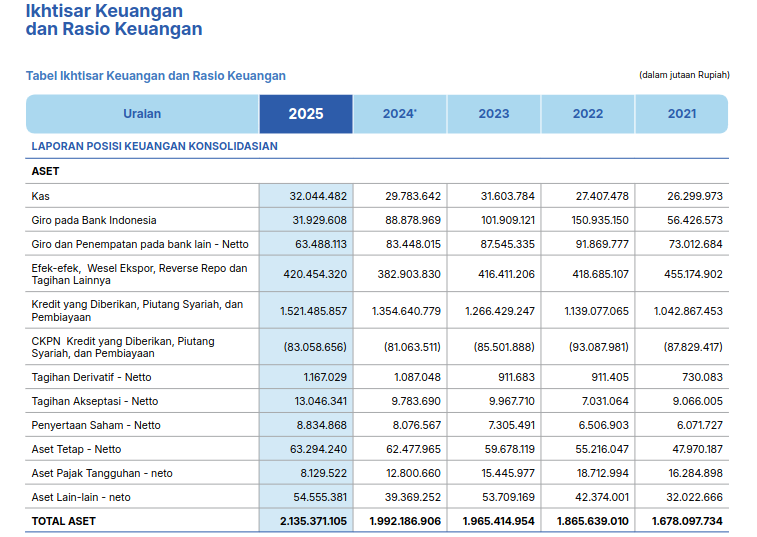
\includegraphics[width=0.9\textwidth]{Images/Cashflow_statement.png}
    \caption{Contoh ikhtisar laporan posisi keuangan konsolidasian yang merepresentasikan struktur aset dan kesehatan fiskal entitas.}
    \label{fig:cashflow}
\end{figure}
Terdapat pula variabel modern lainnya sepeti analisis sentimen berita dan data jaringan sosial yang turut memberikan gambaran mengenai potensi saturasi nilai aset di dalam ekosistem pasar yang sangat dinamis \cite{freitas_game_2024, gong_quantum_2025}.

\subsection{Representasi Data pada Pergerakan Harga}
Analisis teknikal merupakan jenis analisa yang berfokus pada pemetaan stokastik aktivitas transaksi ke dalam domain visual untuk memberikan identifikasi pola-pola harga yang sering kali berulang dalam periode waktu tertentu \cite{freitas_game_2024}. Terdapat berbagai jenis representasi grafis, mulai dari grafik garis hingga \textit{candlestick} yang mana digunakan sebagai instrumen untuk mereduksi (\textit{price noise}) harga yang acak menjadi bentuk visual bagi para analis pasar profesional. Prinsip utama dari Metodologi ini didasarkan pada prinsip bahwa harga pasar saat ini telah mencerminkan secara sempurna seluruh informasi historis serta aksi kolektif para pelaku pasar di masa lampau \cite{schwert_chapter_2003}. Visualisasi data tersebut dapat membantu agen ekonomi dalam melakukan ekstrapolasi tren masa depan berdasarkan pengenalan pola-pola geometris yang telah sering terbukti secara statistik dalam historis perdagangan \cite{sikalo_efficient_2022}.

Secara mikro, pergerakan data pasar finansial direpresentasikan lewat \textit{order book} dan ringkasan harga yang menangkap interaksi antar partisipan pasar secara \textit{real-time}. \textit{Bid-ask spread}, sebagaimana diilustrasikan pada Figure \ref{fig:bid_ask}, merepresentasikan celah harga antara penawaran beli tertinggi dan permintaan jual terendah yang berfungsi sebagai indikator kritis terhadap tingkat likuiditas pasar.
\begin{figure}[htbp]
    \centering
    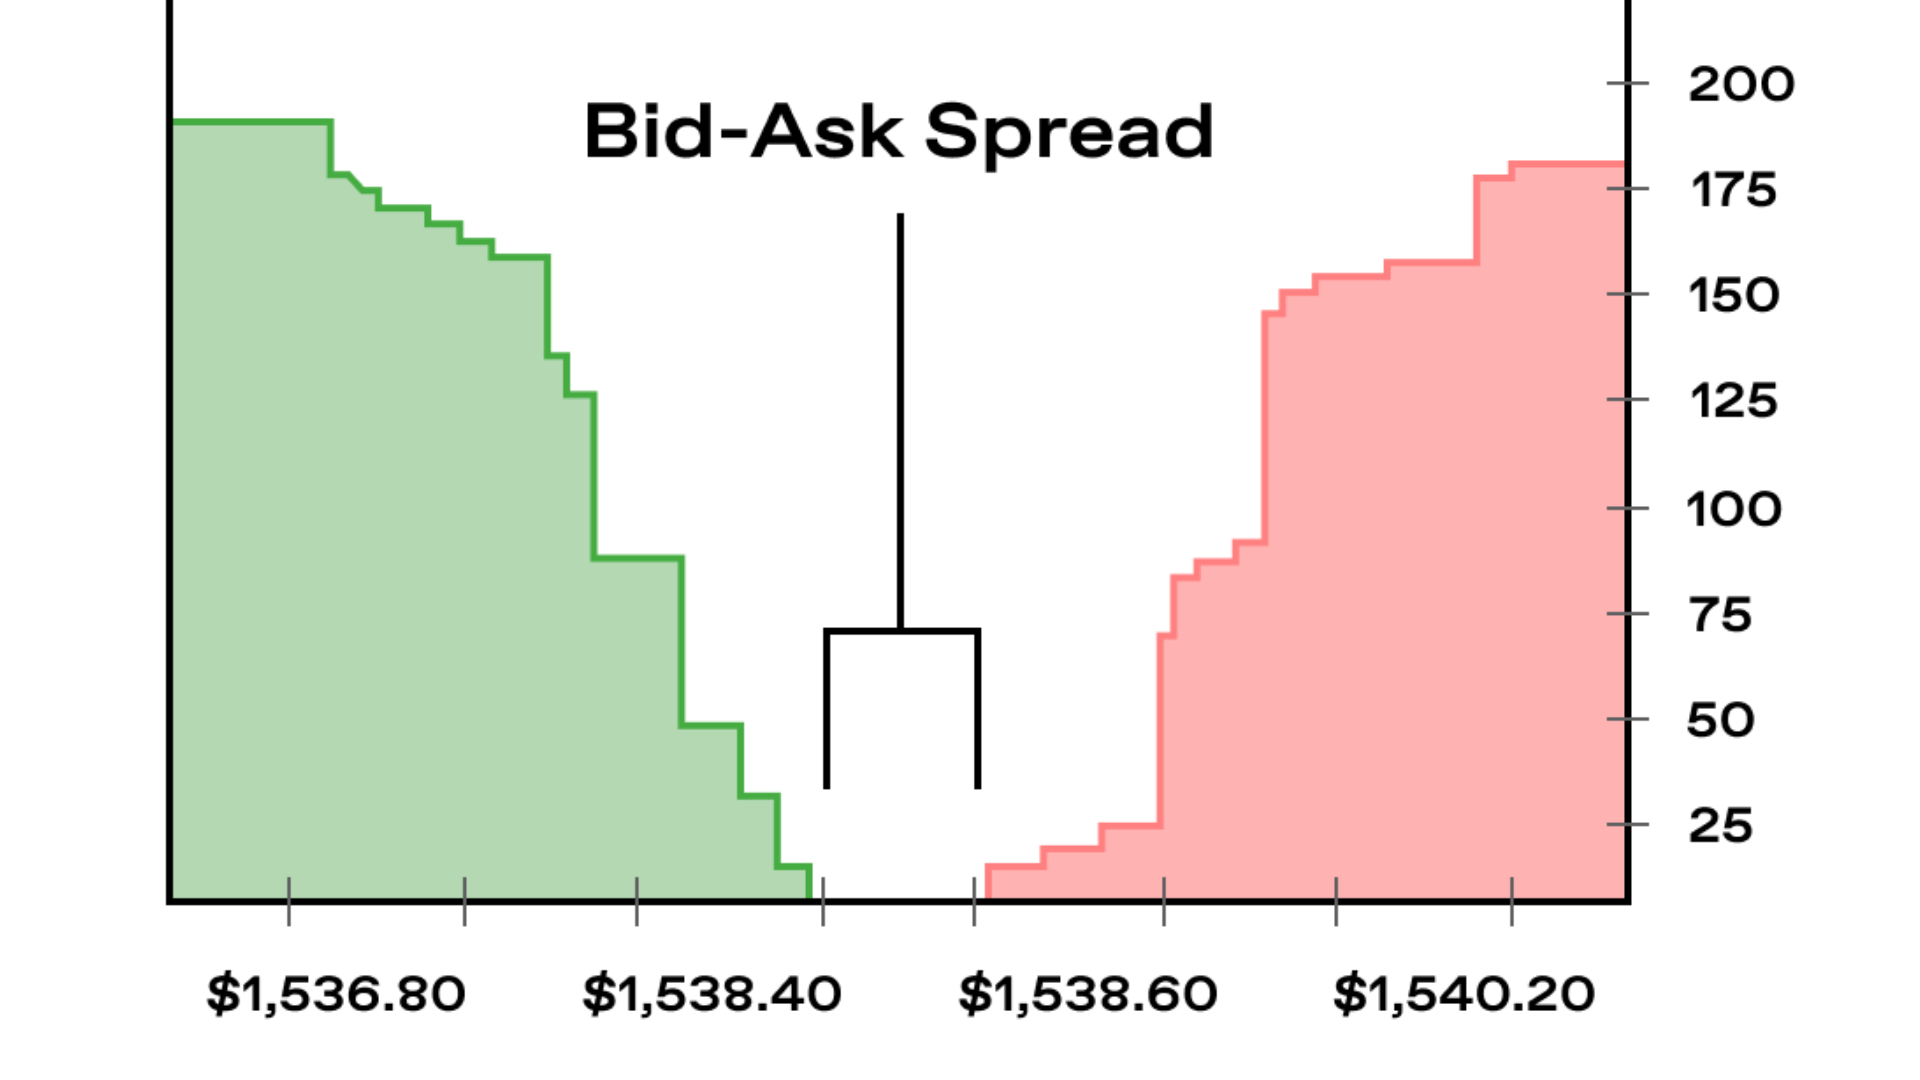
\includegraphics[width=0.7\textwidth]{Images/bid_ask.png}
    \caption{Ilustrasi \textit{bid-ask spread} sebagai representasi friksi transaksi dan likuiditas dalam buku pesanan.}
    \label{fig:bid_ask}
\end{figure}
Representasi \textit{candlestick} yang ditunjukkan pada Figure \ref{fig:Candle1} memberikan visualisasi pergerakan harga dalam interval waktu tertentu yang mencakup nilai \textit{open}, \textit{high}, \textit{low}, dan \textit{close}.
\begin{figure}[htbp]
    \centering
    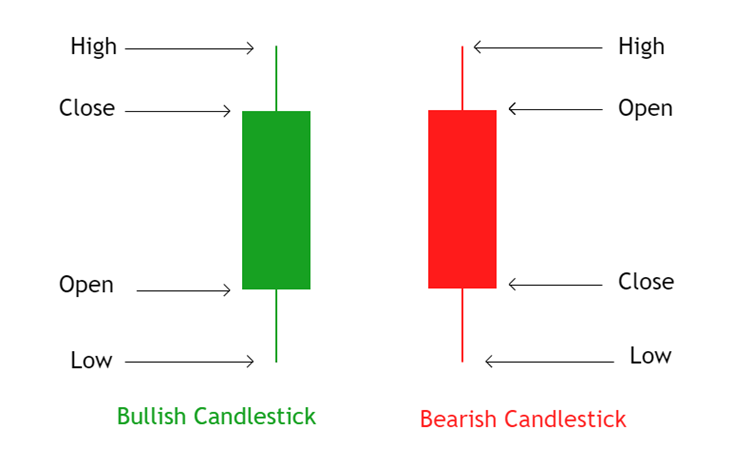
\includegraphics[width=0.7\textwidth]{Images/Candle1.png}
    \caption{Struktur anatomi \textit{bullish} dan \textit{bearish candlestick} yang merangkum fluktuasi harga dalam satu periode waktu.}
    \label{fig:Candle1}
\end{figure}
Berbagai macam representasi data tersebut dimanfaatkan oleh para agen untuk mengevaluasi tekanan beli maupun jual yang sangat penting dalam mengidentifikasi potensi pembalikan atau kelanjutan tren berdasarkan distribusi harga.

Pola harga yang terbentuk secara visual melalui instrumen grafik teknikal pada dasarnya merupakan manifestasi dari psikologi massa serta perilaku kolektif dalam interaksi antar agen di pasar finansial \cite{freitas_game_2024}. Fenomena teknikal seperti level \textit{support} dan \textit{resistance} mencerminkan titik memori sosial di mana para agen cenderung menunjukkan reaksi psikologis yang serupa terhadap ambang batas harga tertentu sehingga menciptakan zona pembalikan arah pergerakan aset yang signifikan. Figure \ref{fig:SnR} mengilustrasikan mekanisme operasional dari batas psikologis tersebut, di mana harga sering kali mengalami pantulan pada level \textit{support} sebelum akhirnya berhasil menembus level \textit{resistance} guna membentuk tren kenaikan yang baru di pasar.
\begin{figure}[htbp]
    \centering
    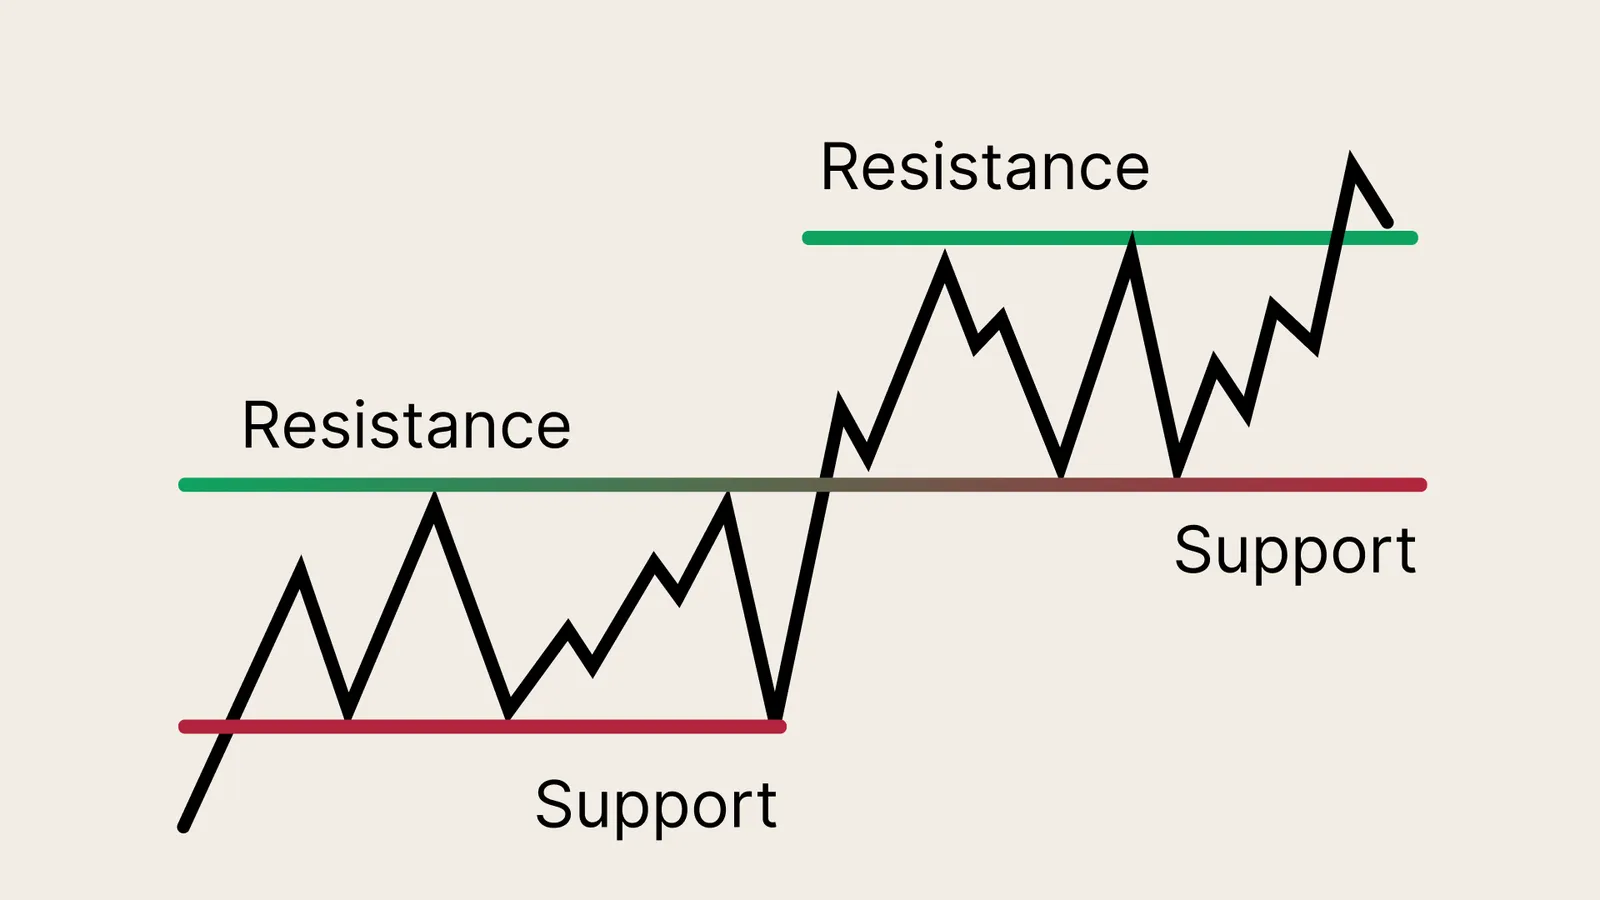
\includegraphics[width=0.8\textwidth]{Images/SnR.png}
    \caption{Representasi visual level \textit{support} dan \textit{resistance} sebagai batas memori sosial dalam dinamika harga aset.}
    \label{fig:SnR}
\end{figure}
Kerangka kontinu dalam data tersebut dapat mempermudah pemodelan kecenderungan sosial melalui pendekatan sosiopsikologi \cite{galam_ising_2010, szabo_evolutionary_2016}. Identifikasi pola teknikal tersebut berfungsi sebagai instrumen untuk mendeteksi fenomena (\textit{herding behavior}) yang menjadi pemicu utama munculnya volatilitas ekstrem dan transisi fase dalam sistem pasar finansial \cite{hidalgo_quantum_2006}.

\subsection{Analisis Kuantitatif Model Markowitz}
Analisis finansial secara kuantitatif dimulai dari proses transformasi data harga mentah menjadi variabel imbal hasil (\textit{returns}) untuk mengurangi efek non-stasioneritas yang sering menghambat analisis statistik. Transformasi tersebut memiliki tujuan menghasilkan data deret waktu yang bersifat stasioner, sehingga berbagai instrumen matematika dapat diimplementasikan secara valid untuk memodelkan perilaku harga di masa depan. Di samping itu, penggunaan imbal hasil logaritmik (\textit{log return}) lebih diutamakan oleh para peneliti karena memiliki sifat memungkinkan agregasi nilai secara matematis serta memberikan kemudahan dalam analisis numerik yang sering kali kompleks \cite{saslow_economic_1999}. Struktur informasi dari data stokastik ini kemudian dianalisis untuk mendekati distribusi normal \cite{hidalgo_quantum_2006}.

Analisis kuantitatif pada model Markowitz bertujuan untuk mencari titik keseimbangan optimal antara ekspektasi imbal hasil dan tingkat risiko melalui seleksi kombinasi aset yang paling efisien secara statistik \cite{markowitz_portfolio_1952}. Dalam penggunaan model ini, investor berupaya untuk menentukan alokasi modal yang tepat pada setiap instrumen untuk memaksimalkan utilitas portofolio berdasarkan tingkat toleransi risiko yang dimiliki oleh agen tersebut \cite{abdul_hali_markowitz_2020}. Penentuan proporsi investasi ini menggunakan perhitungan matematis yang kompleks untuk memetakan interaksi antar aset ke dalam sebuah fungsi biaya yang mencerminkan risiko sistemik pasar secara keseluruhan. Data kuantitatif yang telah didapatkan melalui proses transformasi harga mentah selanjutnya dianalisis lewat fungsi biaya tersebut.

Fungsi biaya dalam model Markowitz menggabungkan beberapa komponen penting seperti matriks kovarians dan ekspektasi imbal hasil. Model tersebut juga menggunakan parameter tingkat toleransi risiko dengan simbol $\lambda$ yang memiliki hubungan berbanding terbalik dengan parameter tingkat penghindaran risiko $\gamma$. Parameter tersebut digunakan untuk menentukan proporsi investasi yang tepat pada setiap instrumen \cite{abdul_hali_markowitz_2020}. Matriks kovarians merepresentasikan interaksi risiko sistemik antar aset yang menentukan derajat volatilitas kolektif, di mana elemen tersebut merupakan inti dari perhitungan risiko dalam manajemen aset modern \cite{markowitz_portfolio_1952}. Struktur fungsi biaya ini memiliki karakteristik kuadratik di mana setiap interaksi antar pasangan aset dihitung berdasarkan korelasi pergerakan harga historis yang telah dinormalisasi dengan \textit{return} maupun \textit{log return}. Fungsi biaya dapat dinyatakan dalam formulasi Lagrangian dalam bentuk persamaan yang mengintegrasikan seluruh parameter tersebut ke dalam satu fungsi objektif
\begin{equation}
\label{eq:lagrangian_markowitz}
\mathcal{L}(\mathbf{\omega}) = \sum_{i,j} \sigma_{ij} \omega_i \omega_j - \lambda \sum_i \mu_i \omega_i
\end{equation}
di mana $\omega_i$ merepresentasikan bobot atau proporsi dana untuk setiap aset $i$, $\sigma_{ij}$ adalah elemen matriks kovarians, dan $\mu_i$ merupakan ekspektasi imbal hasil aset. Pencarian portofolio yang optimal secara teknis setara dengan upaya sistematis untuk menemukan konfigurasi bobot aset yang mampu meminimalkan risiko total pada target tingkat imbal hasil tertentu.

Model pada persamaan (\ref{eq:lagrangian_markowitz}) sering disebut sebagai model \textit{Mean-Variance Portfolio Optimization}. Pada dasarnya, model ini bekerja dengan mengidentifikasi kumpulan solusi yang dikenal sebagai titik-titik \textit{Pareto Optimum} dalam ruang dimensi antara risiko dan ekspektasi imbal hasil. Titik-titik optimal tersebut kemudian membentuk kurva \textit{Efficient Frontier} sebagaimana divisualisasikan secara mendetail pada Gambar \ref{fig:efficient_frontier}. Konsep tersebut sering digunakan sebagai acuan \textit{trade-off} antara risiko dan imbal hasil bagi investor rasional dalam mengoptimalkan portofolio investasi mereka di tengah ketidakpastian pasar.
\begin{figure}[htbp]
    \centering
    
\includegraphics[width=0.8\textwidth]{Images/Efficient_Frontier.png}
    \caption{Kurva \textit{Efficient Frontier} dan \textit{Capital Market Line} sebagai representasi batas efisiensi alokasi aset dalam kerangka kerja model Markowitz.}
    \label{fig:efficient_frontier}
\end{figure}
Bagi para investor institusional, kurva \textit{Efficient Frontier} bertindak sebagai acuan \textit{benchmark} dalam mengevaluasi efektivitas alokasi aset yang mereka gunakan di tengah kondisi pasar yang berfluktuasi secara dinamis \cite{markowitz_portfolio_1952}. Pemilihan titik pada kurva efisiensi ini sangat bergantung pada preferensi investor serta profil risiko manajer investasi untuk mencapai utilitas maksimal. Namun, implementasi model biner dalam seleksi aset dapat meningkatkan kompleksitas navigasi di sepanjang kurva efisiensi karena transformasi masalah tersebut menjadi struktur \textit{Quadratic Unconstrained Binary Optimization} (QUBO) yang akan dibahas pada bab \S\ref{sec:hamiltonian_ising}. 